%%%%%%%%%%%%%%%%%%%%%%%%%%%%%%%%%%%%%%%%%%%%%%%%%%%%%%%%%%%%%%%%%%%%%%%%%%%%%%%%%%%%%%%%%%%%%%%%%%%%%%%%%%%%%%%%%%%%%%%%

\documentclass{llncs}

%%%%%%%%%%%%%%%%%%%%%%%%%%%%%%%%%%%%%%%%%%%%%%%%%%%%%%%%%%%%%%%%%%%%%%%%%%%%%%%%%%%%%%%%%%%%%%%%%%%%%%%%%%%%%%%%%%%%%%%%
\usepackage{calc}
\usepackage{showframe}

\usepackage[lighttt]{lmodern}

\usepackage[british]{babel}%

\usepackage{subcaption}
\captionsetup{compatibility=false}%

\usepackage{cleveref}%
\usepackage[numbers]{natbib}

\newlength\listinglinewidth
\setlength\listinglinewidth\linewidth
\addtolength\listinglinewidth{-0.5cm}

\usepackage{listings}

\lstset{language=python}
\lstset{lineskip=-4pt}
\lstset{linewidth=\listinglinewidth}
\lstset{xleftmargin=0.25cm}
\lstset{basewidth=0.5em}
\lstset{basicstyle=\ttfamily\footnotesize}
\lstset{keywordstyle=\ttfamily\bfseries}
\lstset{frame=single}

\usepackage{pgf}

\newcommand{\picalc}{\(\pi\)-calculus }

\hyphenation{}

%%%%%%%%%%%%%%%%%%%%%%%%%%%%%%%%%%%%%%%%%%%%%%%%%%%%%%%%%%%%%%%%%%%%%%%%%%%%%%%%%%%%%%%%%%%%%%%%%%%%%%%%%%%%%%%%%%%%%%%%

\title{Modelling Realistic User Behaviour in Information Systems as Simulation Aspects}

\titlerunning{}

\author{Tom Wallis\orcidID{} \and Tim Storer\orcidID{}}

\authorrunning{Wallis and Storer}

\institute{University of Glasgow, Glasgow, Scotland,\\
  \email{w.wallis.1@research.gla.ac.uk},\\
  \email{timothy.storer@glasgow.ac.uk},
}

%%%%%%%%%%%%%%%%%%%%%%%%%%%%%%%%%%%%%%%%%%%%%%%%%%%%%%%%%%%%%%%%%%%%%%%%%%%%%%%%%%%%%%%%%%%%%%%%%%%%%%%%%%%%%%%%%%%%%%%%

\begin{document}

%%%%%%%%%%%%%%%%%%%%%%%%%%%%%%%%%%%%%%%%%%%%%%%%%%%%%%%%%%%%%%%%%%%%%%%%%%%%%%%%%%%%%%%%%%%%%%%%%%%%%%%%%%%%%%%%%%%%%%%%

\maketitle

%%%%%%%%%%%%%%%%%%%%%%%%%%%%%%%%%%%%%%%%%%%%%%%%%%%%%%%%%%%%%%%%%%%%%%%%%%%%%%%%%%%%%%%%%%%%%%%%%%%%%%%%%%%%%%%%%%%%%%%%

\begin{abstract}
A workflow model of an information system necessitates modelling the contingent interaction between technology and its 
users. As a result, these models necessarily lie on a spectrum from modelling only the expected interaction, and the 
this interaction together with all possible deviations. Models increase in their complexity as more caveats are 
included.
However, different behaviours often vary due to the same underlying factors: a single flaw in a real-world agent's 
execution of a workflow can manifest in a myriad of ways. This paper shows that an agent's variance is a cross-cutting
concern which can be separated from the workflows they follow. This is explored through the development and application
of a modelling tool which introduces variance to an idealised workflow model. We show that the tool is able to exploit 
this separation of concerns between ideal behaviour and deviation to produce simple workflow models which still exhibit 
contingent behaviour.
\end{abstract}

%%%%%%%%%%%%%%%%%%%%%%%%%%%%%%%%%%%%%%%%%%%%%%%%%%%%%%%%%%%%%%%%%%%%%%%%%%%%%%%%%%%%%%%%%%%%%%%%%%%%%%%%%%%%%%%%%%%%%%%%

\section{Introduction}
\label{sec:introduction}

%%%%%%%%%%%%%%%%%%%%%%%%%%%%%%%%%%%%%%%%%%%%%%%%%%%%%%%%%%%%%%%%%%%%%%%%%%%%%%%%%%%%%%%%%%%%%%%%%%%%%%%%%%%%%%%%%%%%%%%%

Information systems are operated within a wider organisational context, characterised by the needs, demands and
behaviours of individual users, interpersonal relationships, organisational structures, business processes, legal or
regulatory standards, and cultural norms \citep{susman1976autonomy,bade07structures,pentland05organisational}.  The
influence of this \emph{socio-technical} interplay on system behaviour (and often failure) has been described in
multiple and diverse case studies of information systems.  Examples of case studies describing socio-technical system
failures include automated emergency vehicle dispatch \citep{robinson96limited}, electronic voting
\citep{lock07observations} and stock market trading systems \citet{cftc-sec10findings}. In each case, system failure
cannot be attributed to either purely user behaviour or information system failure, but instead to an interplay between
both factors within the overall socio-technical system.

Our contention is that these failures arise because systems engineers lack the tools and methods to efficiently model
and simulate the interaction between the information systems and their organisational context, which comprise a socio-
technical system. Without these facilities, systems engineers cannot predict potential socio-technical system
behaviour, during information system design. Simulating this interaction between the information system and users is
hard because user behaviour is heterogeneous, contingent and evolutionary.  Different users have different abilities,
training and experiences and can experience phenomena such as distraction, misjudgments, exhaustion and confusion that
can have significant influence on how and when a user completes a task.  For example, a novice developer working within
a large team may be unaware of software development best practices described in a workflow, perhaps forgetting to make
frequent commits to a version control server.  Conversely, an experienced developer may omit steps, such as peer reviews
of their code, they consider unnecessary to optimise their performance.

Information system users may also adapt their behaviour due to contingencies that arise due to faults in the information
system, the behaviour of other users or the environment \citep{sommerville09deriving}.  In our example scenario, a
software development team may begin reducing quality assurance efforts as a deadline for a release approaches, in an
effort to ensure all required features are completed \citep{beck02test}. Behavior is also continually evolving, as the
autonomous actors in a system adapt to new circumstances, discover optimizations to their workflows, adapt the workflow
to suit local organizational priorities or take shortcuts
\citep{anderson04heterogeneous,bonen79evolutionary,lyytinen2008explaining}.  In the example scenario, it is reasonable
to anticipate that a novice developer's behaviour will gradually evolve into that of an expert as they gain more
experience.As a consequence, the de facto behavior exhibited within a system may differ from that envisaged by system
architects in idealized workflows.

A system architect must model their workflows as they are intended to be executed in practice, yet due to their
organisational context any information system expresses contingent properties which are fundamental to their accurate
simulation. Conventional systems engineering notations for describing user behaviour, such as BPMN \citep{omg2011omgbpmn},
activity diagrams \citep{omg07omguml} and YAWL \citep{hofstede2010yawl} lack features for efficiently modelling these
characteristics.  Attempting to model the heterogeneity, contingency and evolution of user behaviour using these
approaches inevitably results in models that are either too abstract or narrow to be informative, or too complex to be
tractable.  Alternative approaches that abstract the complexity of user behaviour, such as i* \citep{yu1995social},
Kaos \citep{werneck2009goreistarkaos} and Responsibility Modelling \citep{sommerville09deriving} lack sufficient detail to
generate executable simulations.

%% TODO What is the insight - link to contributions

The key insight of this paper is that the same deviation in behaviour often affects a number of possible actions.
Conversely, a given user's behaviour is a composition of their expected behaviour and the set of irregularities that
affect how the specific user exhibits that behaviour.  Therefore, \emph{we propose and demonstrate the separate
modelling of behavioural irregularities from workflows themselves, showing that they are cross-cutting concerns which can
be applied to an idealised workflow model}.

Specifically, in this paper we present:

\begin{itemize}

\item A method --- and supporting software framework --- for simulating socio-technical systems that allows for the separate
  modelling of idealised workflows and the effects of contingent human behaviours on those workflows.  We use an
  aspect-oriented technique \citep{filman01aspect} to model the effects of variable human behaviour on the execution of
  workflows.  Within an aspect, the method uses a dynamic code-fuzzing \citep{takanen08fuzzing} technique to represent
  alterations to the description of an idealised workflow during execution.

\item A demonstration of the efficacy of the framework in a case study comparison of Waterfall and Test Driven
  Development (TDD) software development workflows.  The case study provides evidence for the industry consensus that
  TDD provides for better software productivity and quality
  \citep{Bhat2006TestDrivenDevelopment,George2004TestDrivenDevelopment,Huang2009EmpiricalTestFirstProgramming}.

  Specifically, the simulation results show that:
	\begin{itemize}
		\item the compared workflows provide for similar outcomes in idealised circumstances
		\item the introduction of contingent behaviour into simulations causes a decline in both productivity and resulting software quality in both workflows
		\item the TDD workflow is more resilient to the occurrence of contingent behaviour than Waterfall.
	\end{itemize}

\end{itemize}

The rest of this paper is structured as follows.  Section \ref{sec:related} discusses related work, covering existing
techniques for modeling socio-technical workflows and the limitations encountered in the literature.  Section
\ref{sec:case-study} introduces the case study problem domain selected to evaluate our approach, and presents the method
for constructing models of socio-technical systems and associated workflows. Section \ref{sec:fuzzing} describes the
development of aspect oriented fuzzing of user behaviour described as workflow models, and the software tool developed for
this purpose.  Section \ref{sec:evaluation} presents our evaluation of the case study and Section \ref{sec:conclusions} discusses conclusions and future work,
as well as noting the potential for applying fuzzing to other forms of socio-technical models.

%%%%%%%%%%%%%%%%%%%%%%%%%%%%%%%%%%%%%%%%%%%%%%%%%%%%%%%%%%%%%%%%%%%%%%%%%%%%%%%%%%%%%%%%%%%%%%%%%%%%%%%%%%%%%%%%%%%%%%%%

\section{Related Work}
\label{sec:related}

%%%%%%%%%%%%%%%%%%%%%%%%%%%%%%%%%%%%%%%%%%%%%%%%%%%%%%%%%%%%%%%%%%%%%%%%%%%%%%%%%%%%%%%%%%%%%%%%%%%%%%%%%%%%%%%%%%%%%%%%

This section presents a literature review of approaches to modelling the interaction between users and information
systems.  Graphical notations have received considerable attention, perhaps due to their perceived efficacy in
communicating specifications between users, customers and system architects.  Workflow description languages, such as as
UML activity diagrams \citep{omg07omguml}, BPMN \citep{omg2011omgbpmn} and YAWL \citep{hofstede2010yawl} can be used to
denote workflows as directed graphs composed of activities.  Various formalisms are used to underpin these notations and
support analysis.  For example, UML activity diagrams are based on Petri Nets, as is BPMN, but with a richer notation
for expressing more complex aspects of activities, such as differentiating between tasks, activities and transactions;
triggering and orchestrating concurrent activities using messages; the identification of information resources need to
realize an activity; and the orchestration of activities across organizational boundaries.  Conversely, YAWL is based on
the \picalc \citep{aalst2004workflow}.  The notation also provides for a richer range of workflow requirements than
activity diagrams, including sophisticated forking and merging rules, separation between workflow specifications and
executions and resourcing and data requirements.

Describing socio-technical behaviour using workflow notations can be difficult, because of the basic assumption that all
contingencies in a workflow can be completely described at a given level of granularity, and that more complex details
can be encapsulated within coarser grained modules.  As argued in Section \ref{sec:introduction}, socio-technical
behaviors are inherently highly coupled with cross cutting concerns, making such refinement based techniques difficult
to apply.  As \citet{israilidis13ignorance} have argued, the `unknowns' in a socio-technical system may be far more
significant than the `knowns'. Several authors have therefore discussed alternative techniques for modeling
socio-technical systems with support for contingent behavior
\citep{dardenne93goal,sommerville09deriving,voinov13integronsters,yu1995social}.

Both i* \citep{yu1995social} and KaOS \citep{dardenne93goal} are goal oriented notations for modeling socio-technical
systems \cite{werneck2009goreistarkaos}.  In contrast to workflows, goal oriented approaches primarily capture what
system actors are seeking to achieve.  Goals can be de-composed into a sub-goal hierarchy using logical operators to
express the form of decomposition. Goals can also be annotated with strategies and/or resource requirements to support
automated analysis.  \citet{yu1995social} argued that socio-technical systems should be viewed as collections of
collaborating actors, each with their own (potentially conflicting) objectives.  Eliciting and analyzing the actor’s
intents allows the inter-dependencies between actors and the overall behavior of the system to be understood, without
the need for explicit models of individual workflows. \citet{herrmann1999vagueness} introduced techniques for annotating
goal oriented system models with vagueness.  The annotation allows for the distinction between consistent vagueness (due
to abstraction) and inconsistent vagueness due to omission.  In principle, this approach allows for the identification
of aspects of a model that are subject to variability.  However, the notation is not accompanied by a formal semantics,
or other means of supporting automated analysis.

Other authors have extended goal oriented approaches to provide greater flexibility. \citet{sommerville09deriving}
argued that stakeholders often struggle to express their behavior within a socio-technical system in terms of goals.
Instead, they argue that the concept of responsibilities, the duties held by an actor in a system, are a more intuitive
means of describing system behaviors that also capture a variety of contingent behaviors.  A notation for expressing the
relationships between responsibilities and resources in order to identify dependencies within a system was provided.
Earlier work on responsibility modeling also provided mechanisms for annotating responsibilities with indicative
workflows, expressing the means by which responsibilities could be executed \citep{dewsbury07responsibility}.  However,
in the case of both goal oriented and responsibility modelling, the ability to document variability in behaviour is not
accompanied with a means of evaluating its effects.

The representation of cross cutting concerns as aspects has been extensively studied in the Software Engineering
literature \citep{Ali2012Aspect}.  However, we are unaware of any research that utilises aspect oriented programming
techniques in simulation models, either for socio-technical user behaviours or elsewhere.  Similarly, the use of code
fuzzing techniques have been employed extensively in quality assurance practices, to assess the impact of variable
behaviour on software systems, including fuzzing of compiler options \cite{fuzzing-compiler}, mutation testing of test
suites \cite{demillo78hints} and fuzzing of inputs test data to search for software security vulnerabilities
\citep{takanen08fuzzing}.  However, we have not discovered any similar work on the application of fuzzing techniques to
dynamically inject variation into a simulation model at runtime.

%%%%%%%%%%%%%%%%%%%%%%%%%%%%%%%%%%%%%%%%%%%%%%%%%%%%%%%%%%%%%%%%%%%%%%%%%%%%%%%%%%%%%%%%%%%%%%%%%%%%%%%%%%%%%%%%%%%%%%%%

\section{Case Study Problem Domain Model}
\label{sec:case-study}

%%%%%%%%%%%%%%%%%%%%%%%%%%%%%%%%%%%%%%%%%%%%%%%%%%%%%%%%%%%%%%%%%%%%%%%%%%%%%%%%%%%%%%%%%%%%%%%%%%%%%%%%%%%%%%%%%%%%%%%%

In this section we introduce our approach to modeling a problem domain and associated idealized workflows in
socio-technical systems.  We have chosen to present the approach through an example case study of team based software
development, in which we will explore the efficacy of two software development lifecycle (SDLC) workflows: Waterfall and
Test Driven Development (TDD).  The case study was chosen as representative of a socio-technical system, combining
different user roles (developer, project manager), information systems (version control server and client) and a variety
of well defined idealised workflows (implementation, testing, debugging etc.).  Further, there is a growing consensus
amongst software development professionals that TDD is a more resilient SDLC than Waterfall to variable human behaviour
\citep{Bhat2006TestDrivenDevelopment,George2004TestDrivenDevelopment,Huang2009EmpiricalTestFirstProgramming}.  The case
study therefore provides an opportunity to test whether the approach presented can be used to distinguish between the
effects of idealised and realistic user behaviours in a socio-technical system.  The modelling approach is implemented
in an agent oriented framework (Theatre\_Ag) written in Python.  Code examples of the case study are provided as
examples, but the full source code is also available for inspection in the case study's repository on GitHub
\cite{storer2016softdev-workflow-scm}.

%%%%%%%%%%%%%%%%%%%%%%%%%%%%%%%%%%%%%%%%%%%%%%%%%%%%%%%%%%%%%%%%%%%%%%%%%%%%%%%%%%%%%%%%%%%%%%%%%%%%%%%%%%%%%%%%%%%%%%%%

\subsection{Problem Domain Model}

%%%%%%%%%%%%%%%%%%%%%%%%%%%%%%%%%%%%%%%%%%%%%%%%%%%%%%%%%%%%%%%%%%%%%%%%%%%%%%%%%%%%%%%%%%%%%%%%%%%%%%%%%%%%%%%%%%%%%%%%

The first step in the modelling approach is to represent the problem domain, describing the inviolable `physics' that
are not subject to variability. An object oriented approach to modeling is adopted \cite{bennett06object}, with
artifacts in the domain implemented as collection of Python classes.  Figure \ref{fig:domain} shows the class diagram
for the problem domain in the case study.

\begin{figure}[t]
  \centering
  \includegraphics[width=12cm]{floats/full-class-diagram-1}
  \caption{Domain model for software development case study, showing artifacts to be manipulated by execution of
    socio-technical workflows.}
  \label{fig:domain}
\end{figure}

A software development effort is hosted on a version control system (VCS) server.  Software developers interact with the
server via VCS client.  Both the server and clients maintain copies of the software system, which must be coordinated
through a VCS update, conflict-resolve, commit cycle.  Software systems are composed of features, representing
user-facing specifications of the system's functionality.  Features may be of varying size, requiring more or fewer code
chunks to be implemented in order to be operational.  Chunks may have dependencies on other chunks in the system.  Each
time a new chunk is added to a feature other chunks may also need to be modified, potentially creating further
dependencies between chunks or introducing bugs.  Bugs may manifest themselves when the feature they are associated with
is operated or exercised through the execution of tests.  Features can be debugged, resulting in the removal of detected
bugs.  Consequently, the more tests created for a feature, the greater the probability of detecting a given bug, easing
the process of debugging a feature or overall system.

The behaviors described above are implemented as methods in the Python classes, as shown in the diagram.  Many of the
effects of these behaviors have side effects which are modeled stochastically. For example, the introduction of bugs and
dependencies during the implementation of a feature occurs with a certain probability. No restrictions are placed on the
implementation of the problem domain classes within the Python language, providing the modeler with significant
flexibility.  For example, operations can accept a variety of arguments, modify object state, invoke operations on other
problem domain classes and return values as desired. The @Property decorator can also be used to improve the readability
of code, as normal.

%%%%%%%%%%%%%%%%%%%%%%%%%%%%%%%%%%%%%%%%%%%%%%%%%%%%%%%%%%%%%%%%%%%%%%%%%%%%%%%%%%%%%%%%%%%%%%%%%%%%%%%%%%%%%%%%%%%%%%%%

\subsection{Workflows}

%%%%%%%%%%%%%%%%%%%%%%%%%%%%%%%%%%%%%%%%%%%%%%%%%%%%%%%%%%%%%%%%%%%%%%%%%%%%%%%%%%%%%%%%%%%%%%%%%%%%%%%%%%%%%%%%%%%%%%%%

In Theatre\_Ag user behaviour workflows are implemented as Python classes, collating related tasks to operate on a
common state. For the purposes of the software development case study, a change management workflow were created for
interacting with a version control server in an update-resolve-commit cycle, as shown as the first class in Figure
\ref{fig:workflows}.  The state for the workflow is the target centralized version control server and a client that
manages the working copy.  Separate task methods are provided for checking out the client, committing working copy
changes to the server and resolving conflicts that arise during a commit task.

\begin{figure}
  \centering
\begin{lstlisting}
class ChangeManagement(object):
    def __init__(self, vcs_server):
        self.vcs_server = vcs_server
        self.vcs_client = None

    @default_cost(1)
    def resolve(self, conflict, rand):
        self.vcs_client.resolve(conflict, rand)

    @default_cost(0)
    def commit_changes(self, rand):
        while True:
            try:
                self.vcs_client.commit()
                self.vcs_client.update(rand)
                break
            except CentralisedVCSException:
                self.vcs_client.update(rand)
                for conflict in self.vcs_client.conflicts:
                    self.resolve(conflict, rand)

    @default_cost(0)
    def checkout(self):
        self.vcs_client = self.vcs_server.checkout()


class Implementation(object):
    def __init__(self, change_management):
        self.change_management = change_management

    @property
    def working_copy(self):
        return self.change_management.vcs_client.working_copy

    @default_cost(1)
    def add_chunk(self, chunk_logical_name, feature, rand):
        feature.extend(chunk_logical_name, rand)

    @default_cost()
    def implement_feature(self, logical_name, rand):
        self.change_management.checkout()

        feature = self.working_copy.get_feature(logical_name)

        while not feature.is_implemented:
            self.add_chunk(len(feature.chunks), feature, rand)
            self.change_management.commit_changes(rand)

    @default_cost()
    def implement_system(self, rand):
        self.change_management.checkout()
        for feature in self.working_copy:
            self.implement_feature(feature, rand)

\end{lstlisting}
  \caption{Python code for workflows describing software implementation and change management.}
  \label{fig:workflows}

\end{figure}

Further workflows were implemented for common software development activities: the Specification and Implementation of
features in the system; Testing; Debugging and Refactoring (reducing dependencies).  Since workflows are modular they
can also be organized hierarchically, so the new workflows make use of the change management workflow, rather than
needing to do re-implement change management for each aspect of development.  Figure \ref{fig:workflows} also shows how
this modularity is exploited for the implementation workflow. In this example, the workflows for modifying the structure
of a software system (for adding chunks or tests and so on) depend on the change management workflow in order to
coordinate the distribution of changes within a team.

Two further workflows, Waterfall and Test Driven Development (TDD) were implemented to investigate the performance of
different team based software development lifecycles (SDLC)when subject to variable behavior.  The Waterfall SDLC
\cite{benington83production} describes a linear staged approach to system development, in which specification of all
features is followed by system implementation, testing, debugging, refactoring and final deployment.  Conversely, TDD
\cite{beck02test} prescribes the definition of tests for each feature, before proceeding to implementation and
refactoring.  Advocates of TDD argue that such an approach results in software that is delivered quicker and of higher
quality because tests are explicitly linked to the specification and features are not committed without a passing test
suite.


%%%%%%%%%%%%%%%%%%%%%%%%%%%%%%%%%%%%%%%%%%%%%%%%%%%%%%%%%%%%%%%%%%%%%%%%%%%%%%%%%%%%%%%%%%%%%%%%%%%%%%%%%%%%%%%%%%%%%%%%

\subsection{Simulation of work in Theatre\_Ag}

%%%%%%%%%%%%%%%%%%%%%%%%%%%%%%%%%%%%%%%%%%%%%%%%%%%%%%%%%%%%%%%%%%%%%%%%%%%%%%%%%%%%%%%%%%%%%%%%%%%%%%%%%%%%%%%%%%%%%%%%

Theatre\_Ag simulations proceed via the execution of tasks in workflows by agents representin the users of the
information system.  A simulation is initiated by configuring a set of actors with an initial set of tasks.  These tasks
are references to methods in workflow instances.  From the initial configuration, execution of a task may result in new
workflow instances being created and tasks being passed to other actors.  Also, the execution of one task in a workflow
may result in other sub-tasks being initiated, so each actor maintains a trace of tasks executed during a simulation in
a tree structure for later inspection.

The Theatre\_Ag framework is designed for simulating socio-technical systems, and so provides for both the explicit
representation of problem domain time for controlling task execution; and concurrent execution of tasks by actors.  Each
agent executes their tasks as a separate thread, but synchronizes on a central clock that measures time in discrete
ticks of domain specific precision.  Task execution proceeds without interruption until a task with cost greater than 0
is encountered.  Task costs are denoted using the \lstinline!@default_cost! decorator in a workflow as shown in Figure
\ref{fig:workflows}.  The actor pauses execution of a task until sufficient ticks from the centralized clock have been
received and then resumes execution.  This mechanism is implemented transparently with respect to workflow classes,
easing the modeling burden for the user.

In the case study, simulations were configured to represent a team of software developers working on a software
project. Simulations were developed for both types of SDLC in the case study.  For Waterfall, the initial configuration
specified an agent in the team with the role of project manager.  This agent is directed to allocate tasks for each
stage of the software development process (specification, implementation, testing, debugging, refactoring) to other
agents in the team and waits for all tasks in each stage of the development process to be complete before allocating
tasks in the next stage.  For TDD, all members of the software development were configured to draw features to be
implemented from the project backlog and implement them following TDD.

%%%%%%%%%%%%%%%%%%%%%%%%%%%%%%%%%%%%%%%%%%%%%%%%%%%%%%%%%%%%%%%%%%%%%%%%%%%%%%%%%%%%%%%%%%%%%%%%%%%%%%%%%%%%%%%%%%%%%%%%

\section{Modelling Variability as Workflows Aspects}
\label{sec:fuzzing}

%%%%%%%%%%%%%%%%%%%%%%%%%%%%%%%%%%%%%%%%%%%%%%%%%%%%%%%%%%%%%%%%%%%%%%%%%%%%%%%%%%%%%%%%%%%%%%%%%%%%%%%%%%%%%%%%%%%%%%%%

The Theatre\_Ag framework provides for the modeling and simulation of idealized socio-technical workflows.  However,
these idealized descriptions do not reflect the variability of real work, and so simulations will not capture the
behaviour of such workflows in realistic conditions. In this section we describe our approach to modeling the effects of
variable behaviour such as confusion and distraction using aspect oriented dynamic fuzzing of task descriptions
implemented as Python methods.  To achieve this, we implemented behaviour fuzzing using our implementation of a
dynamic fuzzing library for Python, PyDySoFu \cite{storer2016pydysofu-scm}. 

PyDySoFu intercepts the invocation of methods in fuzzed classes at runtime.  Each time a method that can be fuzzed
executes, PyDySoFu pauses execution and searches a user provided dictionary of advice for a suitable fuzzing aspect. The
aspect is a function that accepts the context (i.e. the Python self reference) of a method invocation and the abstract
syntax tree of the body of the method to be invoked.  The aspect may access and/or alter the context if desired and
return an altered method body.  If an aspect is found, PyDySoFu constructs the abstract syntax tree for the method body
and passes this and the method context to the aspect to obtain the fuzzed method body as an AST.  PyDySoFu then
recompiles the code object for the method from the fuzzed AST and resumes execution.  Further implementation details are
omitted for brevity, but the full source code is available in the project repository for inspection
\cite{storer2016pydysofu-scm}. PyDySoFu is accompanied by a library of aspects from which more complex aspects can be
constructed and parameterized.  This library includes aspects for removing steps, inserting extra steps, applying an
aspect conditionally, replacing conditions, filtering steps to apply another aspect, recursing into control structures
and applying sequences of aspects to a single method.

In order to evaluate the feasibility of our approach, we implemented an aspect that mimics \emph{distraction} in using
the PyDySoFu library.  The distraction aspect represents variable behavior when an actor engaged in one task becomes
distracted by another, irrelevant activity.  The probability of distraction increases as the simulation proceeds,
i.e. the probability of moving to an irrelevant task increases the longer a simulation has been executing.  For example,
a software developer implementing a feature may be distracted by a technology news site as they proceed to later
activities in the workflow.  Conversely, the aspect also allows the probability of distraction to be reduced by
increasing the concentration of an actor (i.e. actors with better concentration do not get distracted as easily).  In
the current work, we do not contend that the implementation of the aspect is empirically accurate, rather that is
representative of a qualitatively recognizable phenomena and that the approach allows for the effect of the phenomena on
a workflow at different severities to be assessed.

The implementation of the \lstinline!incomplete_procedure! fuzzing aspect is shown in Figure
\ref{fig:distraction-fuzzer}.  The fuzzing aspect is parameterized, so the actual aspect is defined inline as
\lstinline!incomplete_procedure!.  The first four lines of the nested aspect configures a probability mass function
(PMF) for choosing how many steps should be removed by the aspect, \lstinline!n!, based on the remaining time in the
simulation and the actor's concentration. The default PMF is shown in the figure, although this can be configured by the
modeler.

\begin{figure}[t]
  \centering
\begin{lstlisting}
def default_pmf(concentration=1.0):

    def _probability_distribution(remaining_time, probability):
        adjusted_probability =\
          probability ** ((remaining_time + 1.0) * concentration)

        return sys.maxint if adjusted_probability == 1.0 \
            else int(1.0 / (1.0 - adjusted_probability) - 1)

    return _probability_distribution

def incomplete_procedure(random, pmf=default_pmf()):

    def _incomplete_procedure(steps, context):
        clock = context.actor.clock
        remaining_time = clock.max_ticks - clock.current_tick

        probability = random.uniform(0.0, 0.9999)

        n = pmf(remaining_time, probability)

        fuzzer =\
          recurse_into_nested_steps(
            target_structures={ast.While, ast.For, ast.TryExcept),
            fuzzer=filter_steps(
              choose_last_steps(n, reapply=False),
              replace_steps_with(
                replacement='self.actor.idling.idle()'
              )
            )
        )
        return fuzzer(steps, context)
\end{lstlisting}
  \caption{An aspect which dynamically truncates the execution of a workflow to represent a distracted user operating a
    system.}
  \label{fig:distraction-fuzzer}
\end{figure}


The next statement defines an aspect that recurses into nested control structures (while, for and try) and applies a
\lstinline!filter_steps! aspect to the bodies of these statements, tail first (i.e. the filter is applied to the most
nested body found first).  The \lstinline!filter_steps! aspect selects up to \lstinline!n! steps to remove from the body
and replaces each of them with an invocation of idle, causing the actor executing the workflow to wait one tick for each
replaced step.  The \lstinline!filter_steps! aspect is then applied successively up through the target AST.  The
\lstinline!choose_last_steps! filter is configured to track how many steps it has already removed, so that the value of
\lstinline!n! is calculated across the entire body of the fuzzed task method, rather than at each level in the
recursion.
 
%%%%%%%%%%%%%%%%%%%%%%%%%%%%%%%%%%%%%%%%%%%%%%%%%%%%%%%%%%%%%%%%%%%%%%%%%%%%%%%%%%%%%%%%%%%%%%%%%%%%%%%%%%%%%%%%%%%%%%%%

\section{Evaluation}
\label{sec:evaluation}

%%%%%%%%%%%%%%%%%%%%%%%%%%%%%%%%%%%%%%%%%%%%%%%%%%%%%%%%%%%%%%%%%%%%%%%%%%%%%%%%%%%%%%%%%%%%%%%%%%%%%%%%%%%%%%%%%%%%%%%%

This section presents the results of applying the socio-technical fuzzing method to the case study.  Evaluating the
correctness of simulation techniques intended for large scale systems is notoriously difficult, as the principle
rationale for developing the simulation is the lack of available empirical observations of the real world phenomena for
use in validation \citet{naylor67verification}.  Our evaluation strategy follows that advocated by Naylor and Finger,
such that we will test and evaluate different observations of the simulation for plausibility.  We will execute the
simulated problem domain in a variety of settings and repeat simulations in order to limit the impact of noise in
observations.  We will also check for example, for plausibility of simulation results in idealized conditions
\cite{shull11assuring} and for results that cannot be possible in the real world \cite{weyuker82testing}.

Simulations of the problem domain were configured as follows.  A single source of randomness was initialized for each
configuration with a seed of 1.0 to provide for repeatability of the experiment and to provide for comparison between
configurations. All configurations were executed for a software development team of 3 actors, with simulations executing
for a maximum of 500 ticks.  Each configuration was run for 25 different projects.  In order to measure the quality of
the development built by the simulation, the system was operated 10 times.  The operation of the simulated development
entails random selection and operation of features for up to 750 features.  If a bug is manifested during operation then
the system halts.  The average trace of the 10 operations of the system was recorded as the system's mean time to
failure (MTF). Software projects consisted of up between 1 and 6 features, with projects divided into small (2 chunks
per feature) and large (4 chunks per feature). Both the Waterfall and TDD SDLC workflows were simulated.  In either
case, the incomplete procedure distraction aspect was applied to either the high level software development workflow, or
to the set of lower level set of development activity workflows (implementation, change management etc.).  The
distraction fuzzing aspect was applied using developer concentration values between 0.001 and 5.0.  Results from the
simulations are stored in the study repository \citep{storer2016softdev-workflow-scm}.

%%%%%%%%%%%%%%%%%%%%%%%%%%%%%%%%%%%%%%%%%%%%%%%%%%%%%%%%%%%%%%%%%%%%%%%%%%%%%%%%%%%%%%%%%%%%%%%%%%%%%%%%%%%%%%%%%%%%%%%%

\subsection{Simulations with no Fuzzing}

%%%%%%%%%%%%%%%%%%%%%%%%%%%%%%%%%%%%%%%%%%%%%%%%%%%%%%%%%%%%%%%%%%%%%%%%%%%%%%%%%%%%%%%%%%%%%%%%%%%%%%%%%%%%%%%%%%%%%%%%

As a first step in evaluating the plausibility of the problem domain representation, configurations where no fuzzing was
applied were considered.  Two hypotheses were developed to test expectations about the problem domain.

It was first hypothesized that there would be an exponential relationship between the size of a project and the number
of commits, due to the number of additional modifications, tests, debugging and refactoring activities that would be
required as the project grew in scale.  Figure \ref{fig:no-fuzzing:features} illustrates that the problem domain
conforms to this expectation, with total number of commits growing exponentially as the project increases in size.  The
plot also distinguishes between small (blue) and large (red) feature projects, showing that the total number of commits
in these types of projects is clearly distinguishable, and that the total number of commits for smaller feature projects
(i.e. with fewer inter-dependencies within chunks) grows more slowly than for larger feature projects.

A second hypothesis considered the relationship between project size and MTF for projects without fuzzing. It was
hypothesized that larger projects would have a lower MTF, because the additional complexity experienced by larger
projects would increase the probability of a bug being manifested.  Again, Figure \ref{fig:no-fuzzing:mtf} confirms this
expectation, with the MTF of projects declining rapidly towards 4000 ticks and then stabilizing.  The stabilization may
occur because refactoring efforts limit inter-feature dependency (and so de-coupling features from one another) but not
intra-feature dependency.

These two assessments suggest the model and workflows developed is plausible and is representative of the problem
domain.  The simplified simulations did not reveal impossible situations, such as larger projects experiencing fewer
commits, or MTF declining below zero.  Similarly, without the application of fuzzing, all projects were fully
implemented and there was little difference between the performance of the Waterfall and TDD SDLCs.

\begin{figure}[t]
  \centering

  \begin{subfigure}{2.3in}
    \fbox{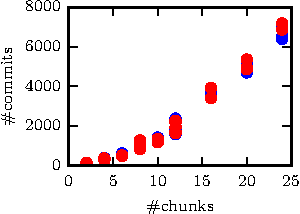
\includegraphics{floats/commits_against_project_size_for_0_fuzz_simulations}}
    \caption{Commits against project size for small (blue) and large (red) feature projects.}
    \label{fig:no-fuzzing:features}
  \end{subfigure}
%  \hfill
  \begin{subfigure}{2.3in}
    \fbox{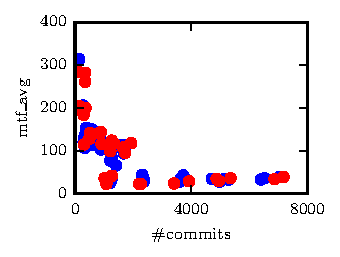
\includegraphics{floats/mtf_against_commits_for_0_fuzz_simluations}}
    \caption{Mean time to failure for Waterfall (blue) and TDD (red) projects.}  
    \label{fig:no-fuzzing:mtf}
  \end{subfigure}
  
  \caption{Scatter plots of software development simulations without fuzzing.}
  \label{fig:no-fuzzing}
\end{figure}

%%%%%%%%%%%%%%%%%%%%%%%%%%%%%%%%%%%%%%%%%%%%%%%%%%%%%%%%%%%%%%%%%%%%%%%%%%%%%%%%%%%%%%%%%%%%%%%%%%%%%%%%%%%%%%%%%%%%%%%%

\subsection{Simulations with Fuzzing}

%%%%%%%%%%%%%%%%%%%%%%%%%%%%%%%%%%%%%%%%%%%%%%%%%%%%%%%%%%%%%%%%%%%%%%%%%%%%%%%%%%%%%%%%%%%%%%%%%%%%%%%%%%%%%%%%%%%%%%%%

We now proceed to compare the performance of the two software development strategies when subject to variable behavior
caused by distraction.  There is a general perception amongst software developers that TDD is a more resilient software
development strategy, although little empirical evidence exists to support this consensus.  Two aspects of the effect of
fuzzing are therefore explored: feature completion and resulting system mean time to failure (MTF).

Figure \ref{fig:fuzzing-features} shows scatter plots for the effect of distraction fuzzing for subsets of workflows.
In both plots, the number of features completed for Waterfall directed projects is plotted in red and in blue for TDD
against the total number of statements removed by fuzzing.  Figure \ref{fig:fuzzing-features:WT} shows the effect when
only the high level software development (Waterfall or TDD) is fuzzed, whereas Figure \ref{fig:fuzzing-features:CTIDR}
shows the effect of fuzzing lower level activities (change management, implementation etc.).  Both figures clearly
demonstrate that in the simulations increasing fuzzing causes a decline in the number of completed features.  However,
in both configurations, TDD is more resilient to distraction fuzzing than Waterfall.

\begin{figure}[t]
  \centering
  \begin{subfigure}[t]{2.3in}%
    \fbox{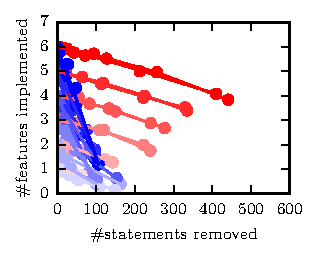
\includegraphics{floats/features_against_total_fuzz_WT}}
    \caption{Fuzzing of Waterfall and Test Driven Development SDLC workflows.}
    \label{fig:fuzzing-features:WT}
  \end{subfigure}
%  \hfill
  \begin{subfigure}[t]{2.3in}
    \fbox{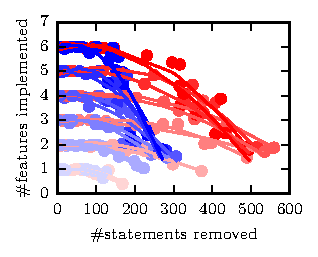
\includegraphics{floats/features_against_total_fuzz_CTIDR}}
    \caption{Fuzzing of Change Management, Testing, Implementation, Debugging and Refactoring workflows.}  
  \label{fig:fuzzing-features:CTIDR}
  \end{subfigure}
  
  \caption{Scatter plots and trend lines of the effect of statements removed on subsets of workflows on feature
    completion. Plots distinguish between Waterfall (blue) and TDD (red).  Smaller project sizes (by feature count) are
    plotted in fainter colors.}
  \label{fig:fuzzing-features}
\end{figure}


For fuzzing of SDLC workflows, the decline in feature implementation appears to be highly linear, with a far steeper
decline for Waterfall than for TDD.  In Figure \ref{fig:fuzzing-features}, both SDLC workflows appear to be largely
immune to fuzzing up to the removal of approximately 100 statements, after which feature completion declines, with
steeper declines for Waterfall.

Figure \ref{fig:fuzzing-mtf} investigates the effect of distraction fuzzing on MTF, again distinguishing between
Waterfall (blue) and TDD (red) SDLCs.  In these plots both fuzzing configurations described in Table \ref{tab:variables}
are combined, as their effects are similar.  Small and large feature projects are plotted separately, as these were
identified as having characteristically different mean time to failures when considering projects without fuzzing.
Similar to the plots of feature completion, the plots of MTF suggest that TDD is more resilient to fuzzing than
Waterfall, which experiences a much more dramatic decline as the number of statements removed increases.  This supports
the contention of advocates that TDD results in higher quality systems because the explicit quality assurance throughout
the life-cycle, rather than only at the end.


\begin{figure}[t]
  \centering
  \begin{subfigure}{2.3in}
    \fbox{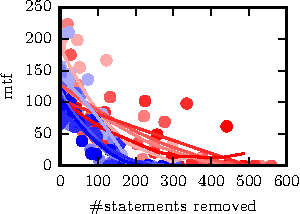
\includegraphics{floats/mtf_against_total_fuzz_projects_small}}
    \caption{Small projects.}
  \end{subfigure}
  \hfill
  \begin{subfigure}{2.3in}
    \fbox{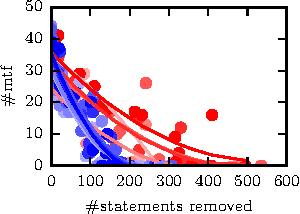
\includegraphics{floats/mtf_against_total_fuzz_projects_large}}
    \caption{Large projects.}  
  \end{subfigure}
  
  \caption{Scatter plots and trend lines of the effect of all fuzzing configurations on the mean time to failure of
    simulated software systems.  Plots distinguish between Waterfall (blue) and TDD (red)..}
  \label{fig:fuzzing-mtf}
\end{figure}
 

%%%%%%%%%%%%%%%%%%%%%%%%%%%%%%%%%%%%%%%%%%%%%%%%%%%%%%%%%%%%%%%%%%%%%%%%%%%%%%%%%%%%%%%%%%%%%%%%%%%%%%%%%%%%%%%%%%%%%%%%

\section{Conclusions}
\label{sec:conclusions}

%%%%%%%%%%%%%%%%%%%%%%%%%%%%%%%%%%%%%%%%%%%%%%%%%%%%%%%%%%%%%%%%%%%%%%%%%%%%%%%%%%%%%%%%%%%%%%%%%%%%%%%%%%%%%%%%%%%%%%%%

This paper has presented and evaluated the use of executable workflow fuzzing to the problem of modeling and simulating
variance in socio-technical system behaviors.  The paper described a proof-of-concept workflow fuzzing tool, Fuzzi\_Moss
and applied it in a case study of software development workflows.  The approach was demonstrated to introduce realistic
variance due to distraction into idealized workflows in accordance with expectations of software development workflow in
practice.

The proof of concept has created a substantial research agenda in the application of fuzzing techniques to
socio-technical system modeling.  In the context of the software development case study, there is a need to understand
why the effects on feature completion and MTF caused by fuzzing were observed.  For example, investigation is needed as
to whether the fuzzing of a particular software development activity, such as change management is the dominant effect
in causing a decline in MTF or feature completion.  Such insights could be invaluable in designing and deploying future
software engineering practices.

More broadly, now that we have validated the approach with an initial case study, more complex socio-technical systems
such as the e-counting system described by \citet{lock07observations} can be considered.  These will provide
opportunities to experiment with a variety of other causes of variability in socio-technical system behavior, such as
subjective misjudgments, exhaustion, misordering of steps and shortcut taking.  Further interdisciplinary research is
required to develop and validate the realism of socio-technical fuzzing aspects that implement these behaviors. There is
a need to link empirical evidence of the causes and occurrence of these behaviors to their impact on the operation of
workflows.

Fuzzing techniques may also be applicable to other socio-technical modeling notations.  For example, fuzzing goal
oriented models such as i* could be used to simulate the shifting goals of actors over time as priorities and focus
varies.  Similarly, fuzzing enterprise modeling techniques such as OBASHI could provide means of assessing the
resilience of critical infrastructures when subject to unexpected behaviors, similar to HAZOPS like techniques that have
been applied manually to responsibility models \citep{lock09modelling}. The proof of concept in this research demonstrates
the potential for the development of realistic simulations of socio-technical systems. The research agenda is towards
simulations that can have predictive capabilities suitable for informing systems engineering decisions before resources
are committed to construction.  The availability of such tools would do much to progress the current craft of large
scale systems engineering.


%%%%%%%%%%%%%%%%%%%%%%%%%%%%%%%%%%%%%%%%%%%%%%%%%%%%%%%%%%%%%%%%%%%%%%%%%%%%%%%%%%%%%%%%%%%%%%%%%%%%%%%%%%%%%%%%%%%%%%%% 

\bibliographystyle{splncsnat}

\bibliography{references,repositories}

%%%%%%%%%%%%%%%%%%%%%%%%%%%%%%%%%%%%%%%%%%%%%%%%%%%%%%%%%%%%%%%%%%%%%%%%%%%%%%%%%%%%%%%%%%%%%%%%%%%%%%%%%%%%%%%%%%%%%%%%





\end{document}
